\begin{tikzpicture}[remember picture,overlay]
    \node[anchor=north west, rotate=0, gray, font=\small] at (-0.75,-7.2) {
    [3] K. Takano, Self-Supervision is All You Need for Solving Rubik’s Cube, 2023
    };
\end{tikzpicture}

\vspace{-5mm}
\begin{itemize}
	\iitem model is trained to predict probability distribution of the source vertex
	\iitem the shorter a path, the more likely it is to occur randomly
	\iitem the cumulative probability $p_1 p_2 \ldots$ of a random training scramble increases as the number of moves decreases.
	\iitem beam search (greedy algorithm) based on cumulative $p$
\end{itemize}
% \vspace{-3mm}

% Fundamental property of combinatorial search: 

\begin{figure}[h]
    \centering
    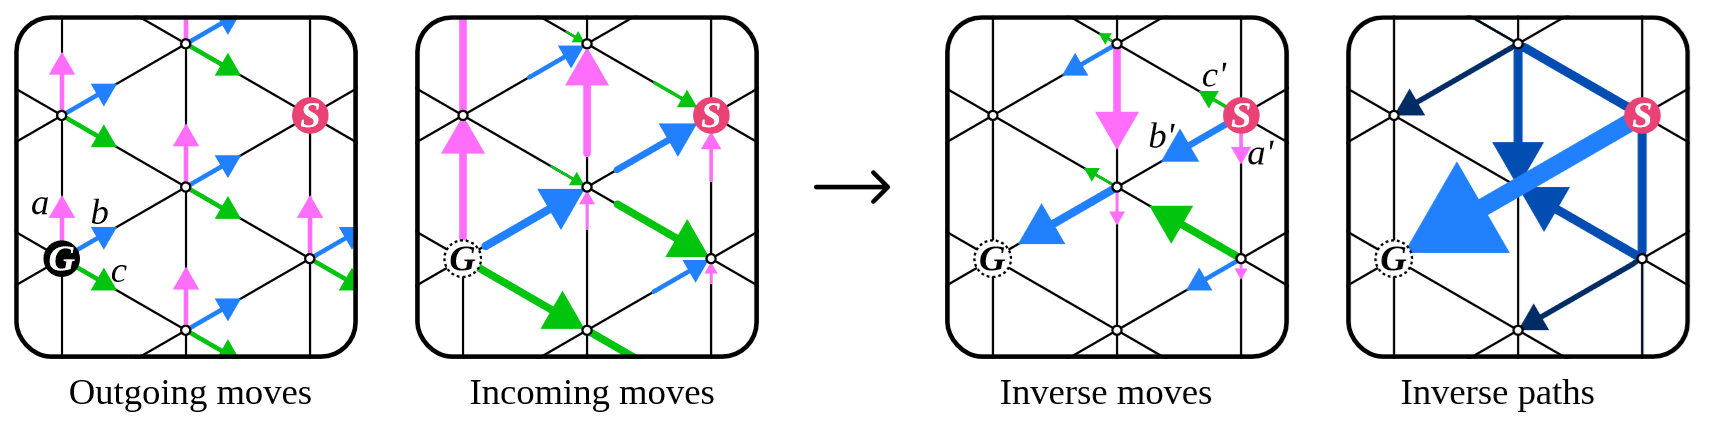
\includegraphics[width=1.0\textwidth]{imgs/unscrambling.png}
    \caption{A miniature instance of combinatorial search with a predefined goal from [3].}
    %\label{fig:}
\end{figure}


